\chapter{An Introduction to Knotted Fields}

\section{Kelvin's vortex atom}
\label{sec:Kelvin}
The original, and perhaps most familiar, example of a knotted field is the smoke ring. Easily made by cutting a circular hole in a rectangular box, then replacing the opposite side entirely with a sheet of rubber, ``a blow on this flexible side causes a circular vortex ring to shoot out from the hole on the other side'' \citep{Kelvin}. In 1867, exactly this demonstration was shown to Lord Kelvin by Peter Guthrie Tait. What is generated is a tightly circulating tube of air, closed into a ring, which propagates stably across the room, rebounding elastically from walls and even other vortex rings (of course to see the ring one first needs to fill the box with smoke, perhaps using dry ice or ``a small quantity of muriatic acid'' \citep{Kelvin}). At the time, the microscopic nature of atoms was still under debate, and the stability of the rings, a consquence of Helmholtz's laws of vortex motion in an ideal fluid \citep{Helmholtz} (translated into English by Tait), coupled with their elasticity and capacity for internal vibration \citep{KelvinMasters, KelvinAMS} prompted Kelvin to suggest that ``Helmholtz's rings are the only true atoms". Kelvin hypothesised that such rings, embedded in a ``perfect homogenous liquid''\footnote{Kelvin did not actually specify whether this fluid was the same as the `ether' hypothesised to transmit electromagnetic waves \citep{KelvinMasters}.}, and ``linked together or ...knotted in any manner'' might form the microscopic basis of all matter \citep{Kelvin}.
\begin{figure}[htbp]
\centering
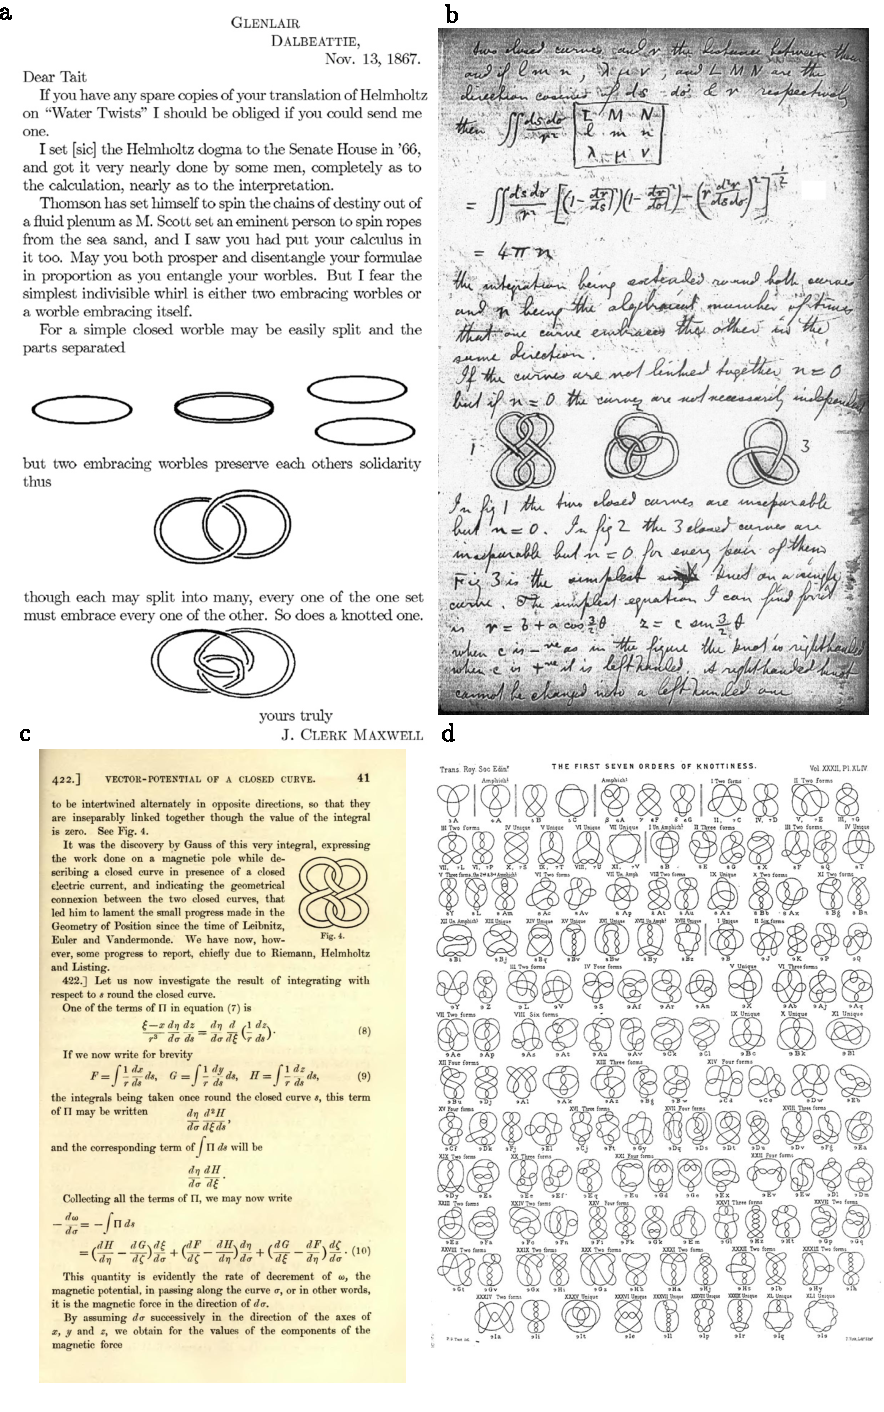
\includegraphics[width=0.99\linewidth]{\IntroductionFigures/History.pdf}
\caption{hi }
\label{fig:History}
\end{figure}

Kelvin's ``vortex atom'' rapidly encountered difficulties in its mathematical content, its falsifiability, and a lack of contempory experimental support \citep{KelvinMasters}. However its content, summarised as ``\textit{Physics = Geometry}'' in Ref. \citep{KelvinAMS}, was compelling (perhaps slightly dangerously so) and apparently motivated Tait, in ``consideration of the forms of knots by Sir W. Thomson's (Lord Kelvin) Theory of Vortex Atoms'', to construct the first systematic tables of knots in 1876--1885 (Figure \ref{fig:History}) \citep{Tait1, Tait2, Tait3}. Tait's articles, alongside a ``very remarkable essay by Listing ... and an acute remark made by Gauss ... with some comments on it by Clerk-Maxwell''~\citep{Tait1} form the initial studies in  what is now the mathematical field of Knot Theory \citep{Lickorish1997}. Maxwell himself, although not an active contributor to vortex atom theory, had a clear interest in the ideas, encouraging Tait and Kelvin to ``prosper and disentangle your formulae in proportion as you entangle your worbles'' (Figure \ref{fig:History}). Indeed the ``comments by Clerk-Maxwell'' referred to by Tait are in fact Maxwell's rederivation of Gauss's Linking number, as presented in his \textit{A Treatise on Electricity and Magnetsim} in 1873, about which we will have much more to say in \S\S\ref{ch2}. 

Despite forming the starting point for modern knot theory, the knotted structures above are quite different to those found in your shoelaces, or in the world of art and design outside the physics department\footnote{or so I am told.}. Rather than a single knotted curve, we have a continuous fluid in whose structure the knot is encoded, and from which dynamical properties of the knot (its motion, stability, a spectrum of vibrational modes etc.) may be derived. More precisely, we have a concentrated tube of vorticity in the fluid, tied into the shape of a knot. Helmholtz's laws of vortex motion demonstrated that, in a perfect (frictionless) fluid this tube of vorticity was `frozen in' to the fluid, unable to dissapate or cross itself. In an idealised vortex atom, the radius of this tube would tend to zero, with the vorticity contained inside becoming infinite, and we would have a singular linelike structure, tied into a knot and embedded into a continuous three dimensional medium. This structure is our first example of what is called a \emph{knotted field}. There is no strict definition of what constitutes of a knotted field, but a sensible effective one is that they are physical fields containing knotted, linked, or otherwise topologically interesting structure, and that this structure has some interplay with the behaviour of the whole field. As we shall see, such fields are not certainly not confined to fluids.

The disconnect between a knotted curve and a knotted field is reflected in Tait's work, which mentions Kelvin's Vortex Atoms briefly as motivation, but focuses in substance on ``\emph{the investigation of the essentially different modes of joining points in a plane}'' \citep{Tait1}. As knot theory developed, its initial connections to hydrodynamics and electromagnetism were further abandoned. We also note that despite the wonderful knot tables produced by Tait (figure \ref{fig:History}) and the reliance of vortex atom theory on knotted and linked vortices, there is no mention above of any experimental evidence of vortices tied in nontrivial knots. 
\begin{figure}[htbp]
\centering
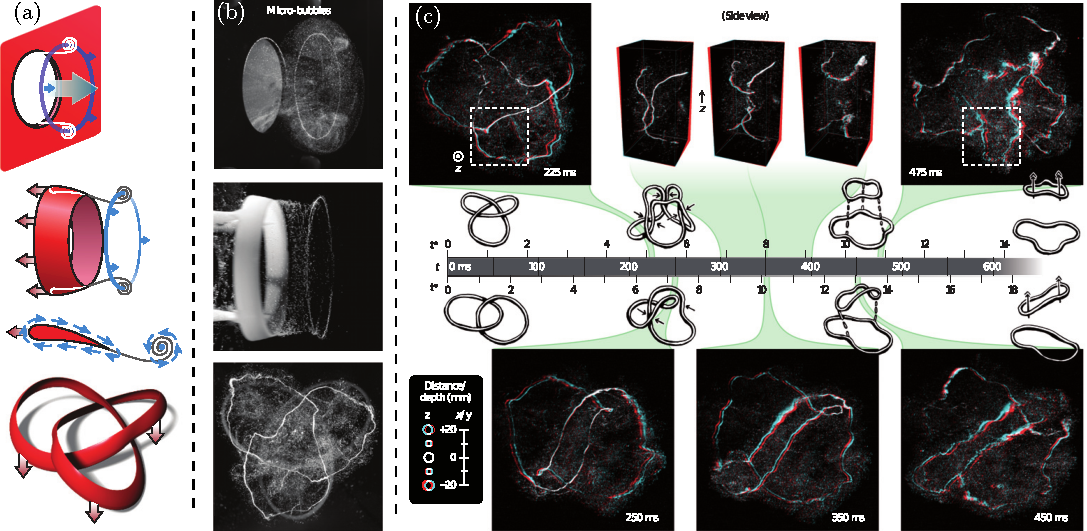
\includegraphics[width=1 \linewidth]{\IntroductionFigures/Irvine_Figs1_3.pdf}
\caption{hi }
\label{fig:Irvine}
\end{figure}

The first experimental construction of nontrivial knotted fluid vortices came 140 years after their initial theoretical investigation, from the Irvine lab in 2013 --- we show in figure \ref{fig:Irvine} several remarkable figures reproduced from Ref.~\citep{Kleckner2013}, in which Kleckner et al. tied a single vortex in water into a trefoil knot, the simplest nontrivial knot, as well as linking two vortex loops together (Kelvin's proposed model for a Sodium atom), before tracking their evolution in full 3D. Ref.~\citep{Kleckner2013} is a noteable example of a more general trend; over the past $\sim10$ years knotted fields have gone from being purely theoretical constructions to being experimentally realisable in a number of systems, and though originally concieved of in fluid dynamics, modern applications are not limited to this context; they have been realised as nodal lines of optical beams~\citep{Dennis2010}, as disclinations in nematic liquid crystals and as spinor Bose-Einstein condensates~\citep{Tkalec2011,Tasinkevych2014,Copar2015}. In the next section we will review the state of modern experiment and theory on knotted fields, beginning with fluids and superfluids --- in some sense the most developed case --- before moving on to parallel developments in liquid crystals and excitable media, which directly underlie the work in \S\S \ref{ch:FitzHughNagumo} and \S\S \ref{ch:TwistBendNematic} in this Thesis. We shall see that the subject has broadened considerably since Kelvin's atoms and the study of fluids. There will be a commonality of ideas between the different disciplines mentioned above, but also geniuine differences.

\section{Modern knotted fields: Fluids}
\label{sec:Fluids}
With the decline of Kelvin's vortex atom theory and the development of knot theory away from its hydrodynamic origins, a resurgence of interest in knotted fields might be dated to the years 1958-1969, with Moreau and Moffatt's seminal papers on Helicity in ideal fluids \citep{Moreau1961,Moffatt1969}, preceded by analogous results in magnetohydrodynamics by Woltjer \citep{Woltjer1958}. Focusing on the ideal fluid, both Moreau and Moffatt independently demonstrated that the Helicity

\begin{equation}
    \mathcal{H} = \int {\bf u} \cdot {\boldsymbol{\omega}} \ d^3 \bf r,
\end{equation}
where ${\bf u}({\bf r},t)$ is the fluid velocity and $\boldsymbol{\omega} = \nabla \times \bf u$ is the vorticity \citep{Saffman1992}, is conserved under the Euler equations of ideal flow. Moffatt in particular gave this invariant a topological interpretation: it measures the linking of vortex tubes within the fluid. Given a fluid where $\omega$ is concentrated along discrete sets of curves $C_i$, Moffat showed that
\begin{equation}
    \mathcal{H} = \sum_{i,j, i\neq j} Lk(C_i,C_j) \Gamma_i \Gamma_j 
\end{equation}
where $\Gamma_i$ is the vorticity flux of along curve $C_i$, and $Lk(C_i,C_j)$ is the Gauss Linking number between curves $C_i, C_j$ (this interpretation of Helicity actually extends to the case where the vorticity is not concentrated along a finite set of curves, but is distributed throughout the fluid \cite{Arnold,Berger,Berger}). Figure \ref{fig:Moffat} shows several examples of vortex tubes with different linking numbers and hence helicities. Seen in this light, the conservation of Helicity is a direct consequence of Helmholtz's laws of vortex motion, and is equivalent to the statement that initially linked vortex tubes remain so; in some sense it is remarkable that the result was not known to Kelvin and Maxwell.
\begin{figure}[htbp]
\centering
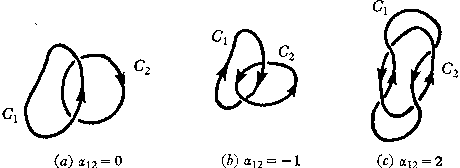
\includegraphics[width=1 \linewidth]{\IntroductionFigures/Moffat.pdf}
\caption{hi }
\label{fig:Moffat}
\end{figure}

When vorticity is not concentrated along a singular curve but distributed in a thin vortex tube, there is additional internal structure --- one imagines a knotted ribbon (Figure \ref{fig:RibbonMontage}(a)), or rubber bicycle tyre (Figure \ref{fig:RibbonMontage}(b)). Flux lines may wind around the centre-line of this tube as in Figure \ref{fig:RibbonMontage}(b), endowing it with a second linking number, the Self-Linking number, which measures the linking of any flux line with the curve centre-line, or equivalently the number of rotations any flux line makes as we traverse the centre-line once. 
\begin{figure}[htbp]
\centering
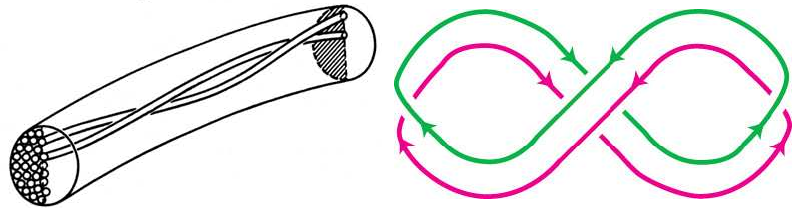
\includegraphics[width=\linewidth]{\IntroductionFigures/RibbonMontage.pdf}
\caption{hi }
\label{fig:RibbonMontage}
\end{figure}
Incorporating this structure into the helicity count we find \citep{Moffat1992}
\begin{equation}
    \mathcal{H} = \sum_{i,j, i\neq j} Lk(C_i,C_j) \Gamma_i \Gamma_j + \sum_{i} \Gamma_i^2 SL(C_i) 
    \label{eq:HelicityCount}
\end{equation}
where $SL(C_i)$ denotes the self linking of each curve $C_i$ with its implicitly assumed ribbon. 

\subsection{Calugareanu's Theorem, Real fluids}
Given a ribbon diagram like figure \ref{fig:RibbonMontage}(a), the self linking number of may be further decomposed as
\begin{equation}
    SL = Tw + Wr.
    \label{eq:Count}
\end{equation}
The first term, the twist $Tw$, counts the local crossings of the ribbon over its centre-line. The second term, the writhe $Wr$, counts non-local crossings of the ribbon over distant parts of the centre line. In figure \ref{fig:RibbonMontage} each crossing of the ribbon over its centre-line is annotated with the nature of its contribution. Note that the $Wr$ count is actually independent of the choice of ribbon. For different diagrams of the same knotted ribbon each of these contributions varies, but their sum $SL$ does not. Averaging over also possible diagrams, i.e. all possible projections of the geniuine three-dimensional curve, one obtains integral formulae for twist and writhe, and in this form the result eq. \ref{eq:Count} was first discovered by Georges Calugareanu \citep{Calugareanu1959,Calugareanu1961} (the interpretation of it given above is however due to Ref.~\citep{Dennis2005}). Calagareanu's Theorem is an important and influential result, finding application in Mathematics, Physics, Biology and beyond. It is of potential relevance whenever one studies the properties of a curve with some internal structure, and so it naturally appears frequently in the study of knotted fields. It will play a role in the curve dynamics studied in \S\S\ref{ch3} and, in its close connection to Maxwell and Gauss's work on linking numbers and electromagnetism, in \S\S\ref{ch2} as well. For the purposes of the current discussion it enables us to speak of \emph{writhe} helicity and \emph{twist} helicity, two seperate contributions to the total helicity count.    

In a real (viscous) fluid, helicity is not \emph{a priori} conserved. The question of whether it is in practice, and the mechanism of its dissipation, are areas of active research and motivation for the experiments shown in Figure \ref{fig:Irvine} \citep{Kleckner2013}. The reconnections shown in figure \ref{fig:Irvine} suggest that helicity is not conserved, however experiments tracking its evolution in detail \citep{Kleckner2013,Scheeler2014,Scheeler2016} find that this is not the case. Instead, reconnections transfer the initial linking of curves (c.f. eq. \ref{eq:HelicityCount}) into self linking, preserving total helicity to a remarkable extent. More precisely, what is conserved is the sum $Lk +Wr$, with the helicity in $Lk$ being transferred to $Wr$ at a reconnection; the twist helicity $Tw$ is dissipated by viscosity (figure \ref{fig:Irvine2}).
\begin{figure}[htbp]
\centering
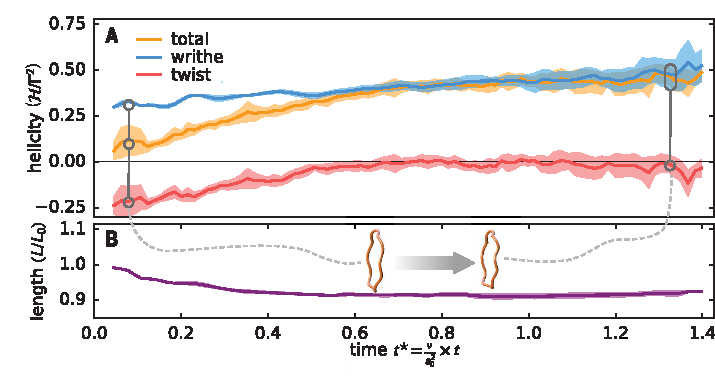
\includegraphics[width=0.7\linewidth]{\IntroductionFigures/Irvine2.pdf}
\caption{hi }
\label{fig:Irvine2}
\end{figure}

\subsection{Fluids as a case study}
The hydrodynamic (and magnetohydrodynamic) story of knotted fields is well developed. We have given a sketch, but the reader is invited to find more detail in reviews such as Refs. \citep{Moffatt2014, Irvine2018}. Outside of hydrodynamics the above discussion acts as a template for what one might expect in knotted fields more generally; a test case which other systems may be compared to and contrasted against. In particular, linking and self-linking of structure occur in a variety of contexts, and in an analogy to (\ref{eq:HelicityCount}) one might seek to connect them to conserved quantites, and use them to understand the dynamics of the entire system under study. To give a brief example of system for which this template is fruitful consider superfluids, close cousins of normal fluids described by a complex scalar field $\psi = |\psi| e^{i \phi}$ (Figure \ref{fig:SuperFluidMontage}(a)) evolving via the non-linear Schroedinger equation \citep{Kleckner2013}. Here vortices are given by singular lines where the circle-valued phase field $\phi$ is undefined, and about which it winds by $2\pi$. As in fluids, one may define some notion of helicity (although its precise form is more ambiguous than is the case in fluids \citep{Salman}), initialise knotted vortices and study their evolution (figure \ref{fig:SuperFluidMontage}(b)) \citep{Kleckner2013,Scheeler2014}. The helicity evolution turns out to be remarkably similar to that of real fluids \citep{Kleckner2013,Scheeler2014}; reconnections occur in a manner similar to thse found in real fluids, and they preserve the combination $Lk+Wr$.  
\begin{figure}[htbp]
\centering
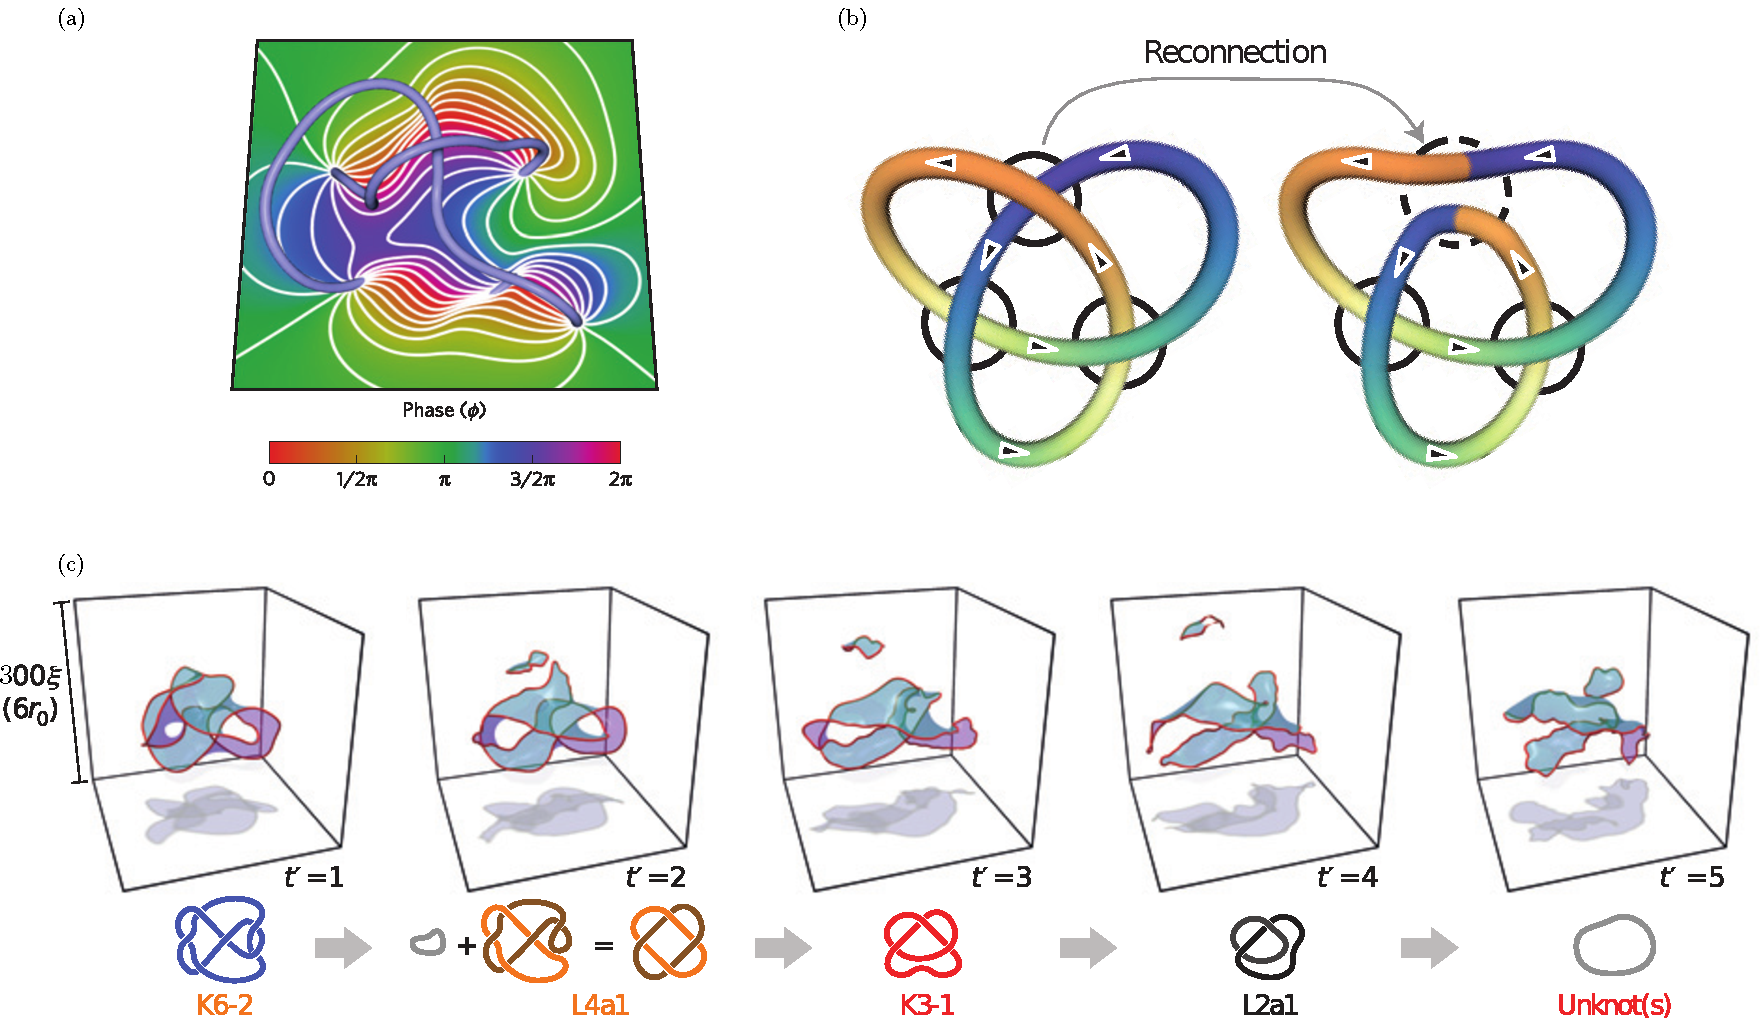
\includegraphics[width=\linewidth]{\IntroductionFigures/SuperFluidsMontage.pdf}
\caption{hi }
\label{fig:SuperFluidMontage}
\end{figure}

However, it is not the case that knotted fields in all other systems may be understood simply through the lens of fluids. In the following section we turn to the second experimental system with which substantial work on knotted fields has been done, the nematic liquid crystal cells of Refs.~\citep{Tkalec2011,Tasinkevych2014,Copar2015}. There will be some crossover with the discussion above, but also geniuine differences, especially in the theoretical constructions involved, which are of a quite different character. 
\section{Modern knotted fields: Liquid Crystals}
\begin{figure}[htbp]
\centering
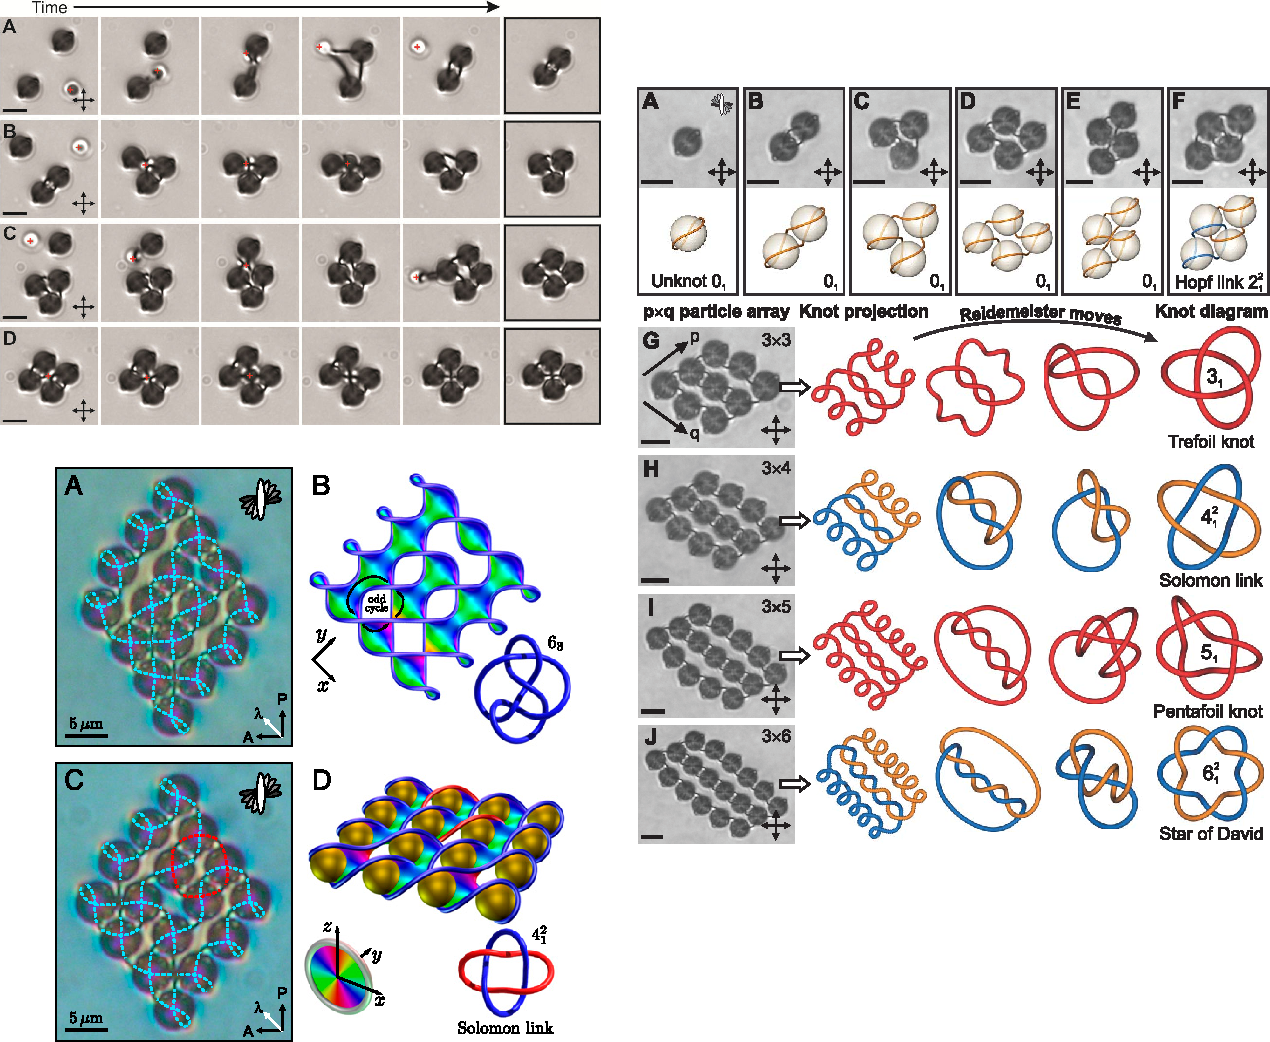
\includegraphics[width=0.8 \linewidth]{\IntroductionFigures/LiquidCrystalMontage.pdf}
\caption{hi }
\label{fig:KnottedLiquidCrystal}
\end{figure}
A second experimentally constructed knotted field is shown in figure \ref{fig:KnottedLiquidCrystal}. It is quite different to that of figure \ref{fig:Irvine}. By including microscopic colloids a few $\mu$m wide into a thin cell of nematic liquid crystal, experimentalists~\citep{Tkalec2011,Tasinkevych2014,Copar2015} are able to force the appearance of defect lines in the material. These defects may then be manipulated with lazer tweezers, and by weaving them about an array of colloids, a knotted field encoding any type of knot or link can be constructed; unlike the fluid vortices above, these structures are stable, able to be experimentally probed in some detail. This system provides a testbed for series of new ideas about knotted fields described below, but first we step back a moment and provide a brief description of what liquid crystals, defects and colloids etc. actually are.

\subsection{A brief introduction to liquid crystals}

Liquid crystals are a class of materials which possess properties associated to both liquids and solids~\citep{deGennes1992}. In their most common form, the nematic phase, they show no positional order, and flow like a liquid . However, they do show orientational order: if one attempts to twist a portion of the liquid crystal it will respond elastically, as a solid would\footnote{This is remarkable: imagine your surprise if, upon attempting to stir your coffee, you found it fiercly resisted your attempts to turn the spoon, but was nevertheless happy to be poured down the sink.}. The microscopic basis for this behaviour comes from the type of molecules which comprise nematics, two examples of which are shown in Figure \ref{fig:DeGennesMontage}; they are typically thin rods which locally align themselves along some common axis without taking on any sort of crystalline postitional order. In continuum theories this orientational order is described by a spatially varying unit vector field $\bf n$, called the director, which represents an average local molecular orientation, as shown in Figure \ref{fig:DeGennesMontage} (c).
\begin{figure}[htbp]
\centering
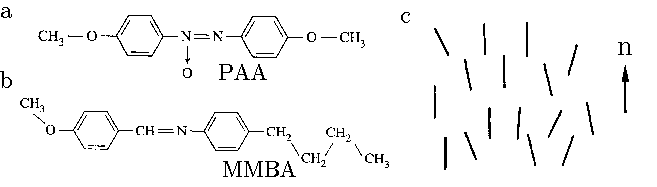
\includegraphics[width=1\linewidth]{\IntroductionFigures/DeGennesMontage.pdf}
\caption{hi }
\label{fig:DeGennesMontage}
\end{figure}

The theory of their elastic distortions contains much interesting geometry which we will return to in \S \ref{sec:Geometry}, but for an understanding of figure \ref{fig:KnottedLiquidCrystal} we instead focus on a celebrated feature of nematics \citep{Frank1958}, their topological defects. If one shines polarised light through a thin slice of nematic placed between crossed polarisers, they will observe something like figure \ref{fig:Disclination}(a), a Schlieren texture \cite{DeGennes1992}. Places in the sample where the director $\bf n$ is aligned with one of the two polariser directions H and V do not transmit light, leading to the dark brushes observed. One immeadiately notes points where the brushes meet, sometimes with two brushes leading into a point, sometimes four. What is the structure of the director at these points? The confluence of dark brushes implies that, in a small circle around these points, the director winds, and that at the point itself we cannot consistently define $\bf n$; these points are topological defects, places where the order breaks down. Traversing such a circle around a point with two brushes, the director is aligned with each of H and V only once; in other words it makes only half a turn in a full circle around the defect. This observation is enough to establish that the director $\bf{n}$ must in fact be non-orientable; it should not be thought of as a vector field, but as a line field, for which $\bf n \sim - \bf n$.
\begin{figure}[htbp]
\centering
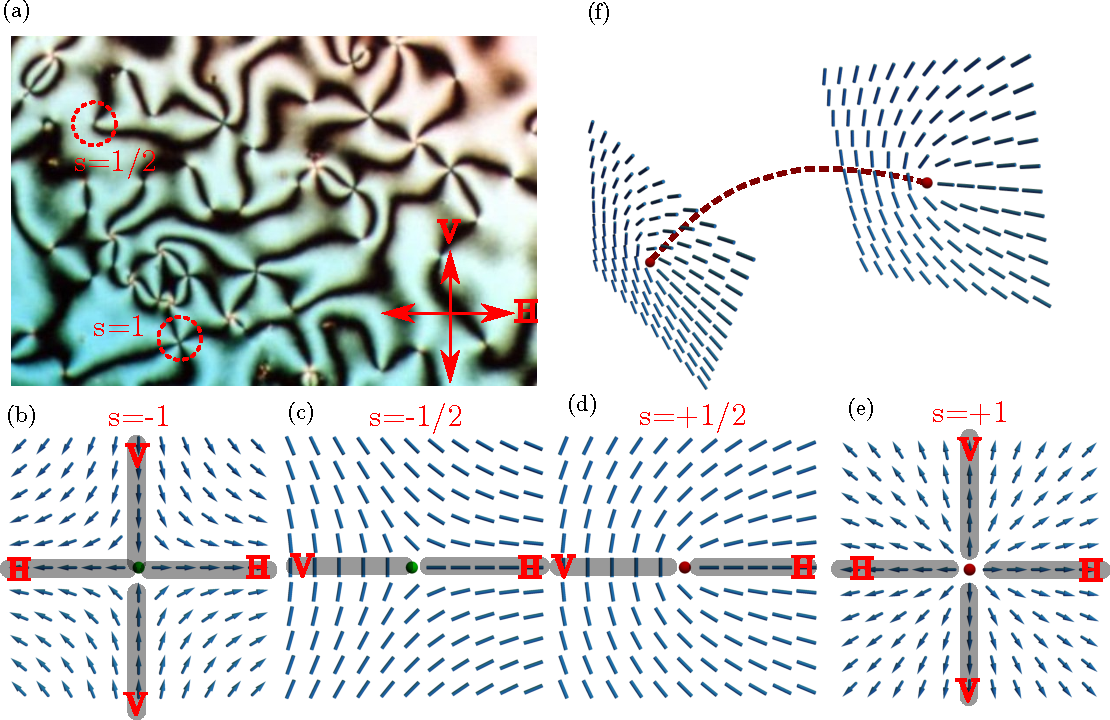
\includegraphics[width=1\linewidth]{\IntroductionFigures/DisclinationLine.pdf}
\caption{hi }
\label{fig:Disclination}
\end{figure}
In figure \ref{fig:Disclination} (b)--(e) we show configurations of the director around these defects, with their associated Schlieren texture brushes. In (b) and (e) we have four brushes, and a line field which can be oriented; to emphasise this fact we have decorated the line field with one of the two possible choices of arrowheads. Figures (c) and (d) correspond to the non-orientable two brush case; here one cannot consistently assign arrowheads to the rods (it is worth trying to imagine doing so). Note that from a single image such as figure \ref{fig:Disclination}(a), we cannot distinguish defects winding in a right handed sense ($+$, in the figure) from left handed by counting brushes.  In two dimensions these defects, also called disclinations or dis\emph{in}clinations \citep{Frank1958}, are points, but in three dimensions they are lines, transverse cross sections of which have local profiles resembling the two dimensional case; a schematic illustration is shown in Figure \ref{fig:Disclination}(f). As with fluid vortices, these disclination lines may be knotted and linked together, and the rotation of the local profile along the disclination (see the cross sections in Figure \ref{fig:Disclination}(f)) provides internal structure giving rise to self linking.

\subsubsection{Experiments on knotted disclination lines}

We now return to the experiments of Refs~\citep{Tkalec2011,Tasinkevych2014,Copar2015}. In contrast to situation in fluids, one of the major advantages of working with liquid crystal disclinations is the control experimentalists have over them. By including microscopic silica spherical colloids (4.72 $\mu$m diamter in figure \ref{fig:KnottedLiquidCrystal}) into a sample of liquid crystal with specific surface anchoring conditions, experimentalists may frustrate alignment of the director $\bf n$ in a controlled fashion, neccesitating the appearance of disclination lines \cite{}. For example, in a thin cell of liquid crystal treated to promote uniform alignment of $\bf n$ within the sample, the inclusion of a colloid with normal anchoring conditions forces the appearance of a defect line around it to cancel the colloid's topological charge (it effectively acts as a point defect) and allow $\bf n$ to relax to uniform at large distances. Two such ``Saturn's ring'' configurations may be seen in the first frame of figure \ref{fig:KnottedLiquidCrystal}(a). Once generated, these disclinations, as well as the colloids they wrap around, may be further manipulated using lazer tweezers \citep{Tkalec2011}, as shown in the remainder of figure \ref{fig:KnottedLiquidCrystal}(a). When two of these colloids are brought together the disclinations, either spontaneously or induced by the tweezers, fuse together (Figure \ref{fig:KnottedLiquidCrystal}(a), top row). Assembling an array of these colloids and weaving the disclination lines around them, the setup of Refs.~\citep{Tkalec2011,Tasinkevych2014,Copar2015} allows targeted construction of any knot or link; examples of some possible link topologies are shown in Figure \ref{fig:KnottedLiquidCrystal} (b). This system strikingly illustrates that knotted fields have more structure than a single knotted curve; the curve organises the entire field (in this case the director $\bf n$) around it. Figure \ref{fig:KnottedLiquidCrystal}(c) shows the knotted liquid crystal coloured by whether the director is twisting in a right or left handed sense. We see that the disclinations separate the liquid crystal into alternately right and left handed regions. In fact this division allows construction of a surface spanning the disclinations called the Pontryagin-Thom (PT) surface \citep{Chen2013,ChenThesis}, shown as the coloured surfaces in figure \ref{fig:KnottedLiquidCrystal}(c), which classifies the topology of this liquid crystal texture; we shall return to it in a moment.

Let us compare the phenomena seen here to \S\ref{sec:Fluids}. In contrast to fluid vortices, it is experimentally possible to stabilise liquid crystal disclinations with colloids. This fact alone leads to many differences in the character of theoretical work on them. In the absence of the stabilising colloids, the disclinations will shrink under effective line tension and undergo reconnections, however there is relatively little theoretical work on possible conservation laws analogous to eq. (\ref{eq:HelicityCount}) or on the structure of these reconnections, although some results do exist \cite{Machon}. In this sense the dynamics of these knotted fields is less understood than is the case in fluids.  It turns out, however, that there is much to be understood even about the statics of knotted liquid crystal fields. Loosely, this may be understood by observing that in a two dimensional fluid there is only one type of vortex, topologically speaking. In a slice of liquid crystal, however, we saw there were many types, indexed by the winding of the director. What of liquid crystal textures in three dimensions? More specifically, given the knotted disclinations shown in figure \ref{fig:KnottedLiquidCrystal}, are the liquid crystal textures corresponding to them unique, or are there many inequivalent possibilites? Questions like these have a long history in liquid crystal physics which, coupled with the difference in experimental possibilites we saw above, makes some split between the character of work on knotted fields in fluids and that in liquid crystals expected.

\subsection{Homotopy theory of knotted disclinations and Pontryagin-Thom surfaces}
The traditional method of understanding liquid crystal textures containing defects is to place a measuring surface around a defect and study the possible textures on this surface, i.e. the different classes of map from the measuring surface to the space of possible values the order takes. Maps are equivalent when a continuous deformation, called a homotopy, exists between them, and as such this framework is known as the homotopy theory of defects \citep{Mermin1979,Alexander2012}. For point defects in a two-dimensional slice of nematic, this is what we did above, using a circle as our measuring surface. There, the space of possible directions $\bf n$ can point in is $S^1/\{x\sim-x\}$, the circle with antipodal points identified, also called the real projective line $\mathbb{R}P^1$. Thus the different classes of texture are reduced to the classification of maps ${\bf n}:S^1 \rightarrow \mathbb{R}P^1$. Actually computing these classes is the work of Algebraic Topology \citep{Hatcher2012}, in which maps of a sphere $S^n$ into a space $X$ are termed the homotopy groups $\pi_n(X)$. It is found that $\pi_1(\mathbb{R}P^1) \approx \mathbb{Z}$ and thus there are infinitely many types of point defect in two dimensions as far as the traditional form of the theory is concerned. In three dimensions, the director takes values in $S^2/\{x\sim-x\}$, the sphere with antipodal points identified, also called the real projective plane $\mathbb{R}P^2$. Encircling a disclination line with a measuring loop as shown in Figure \ref{fig:RP2}, we compute $\pi_1(\mathbb{R}P^2) \approx \mathbb{Z}_2$, and thus there are precisely two distinct types of disclination\footnote{ One understands this difference by allowing the director in figures \ref{fig:Disclination} (b) and (c) to buckle out of the plane of the paper, reducing these textures to the trivial one. This ``escape in the third dimension'' causes $\mathbb{Z}$ to undergo a mod 2 reduction.}.
\begin{figure}[htbp]
\centering
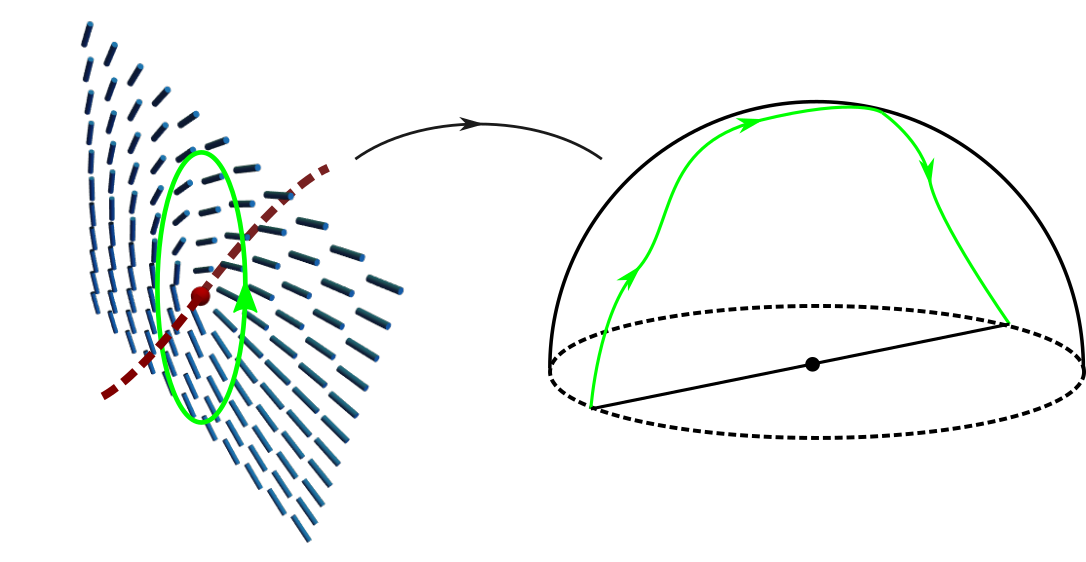
\includegraphics[width=0.9\linewidth]{\IntroductionFigures/RP2.png}
\caption{hi }
\label{fig:RP2}
\end{figure}

A limitation of this approach is that, in only considering the texture on a specific measuring surface (in practice a sphere of some dimension) it discards information about the rest of the texture, which leads to ambiguities when considering multiple defects or more complex structures such as knotted and linked disclinations \citep{Alexander2012,MachonThesis,Machon2014,Machon2016}. A more recent, global approach \citep{MachonThesis,Machon2014,Machon2016} does not fix a measuring surface, but instead classifies maps into $\mathbb{R}P^2$ where the domain is the entire liquid crystal sample $M$ minus some set of (possibly knotted and linked) disclination lines $L$. The result is that the homotopy classes of the director are given by
\begin{equation}
[M-L, \mathbb{R}P^2] \approx H_1(\Sigma(L); \mathbb{Z})/\{ x \sim -x\}
\label{eq:HomotopyClassification}
\end{equation}
where $\Sigma(L)$ is the branched double cover of the link complement (its appearance in the result is a consequence of director non-orientability), and $H_1(\Sigma(L); \mathbb{Z})$ is its first homology group. Without going into the details of this result, it is clear that these homotopy classes are far richer than the traditional classification scheme for disclinations would suggest, and that they depend strongly on the knot or link under consideration. To illustrate this point, in figure \ref{fig:MachonMontage} we reproduce a `periodic table' of possible textures for $(p,q$) torus links from Ref.~\citep{MachonThesis}. Taking the simplest example from this table we see that for the Hopf Link, consisting of two curves passing through each other once and given by $(p,q)=(2,2)$, there are exactly two nonhomotopic textures. Returning to the knots shown in figure \ref{fig:KnottedLiquidCrystal}, for each knot there many be multiple nonhomotopic textures, and the knot diagram alone does not tell us which has actually been made. How should we extract this information, and visualise distinct textures? In \ref{fig:DisclinationLine} simple pictures of the director in the vicinty of a defect prove informative, but the same cannot be said of a swarm of sticks in three dimensions.
\begin{figure}[htbp]
\centering
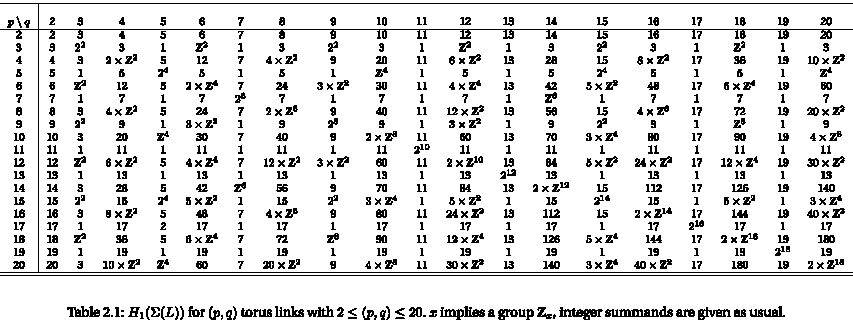
\includegraphics[width=\linewidth]{\IntroductionFigures/MachonMontage.pdf}
\caption{hi }
\label{fig:MachonMontage}
\end{figure}

One solution is a construction which generalises the dark brushes of Schlieren textures to three dimensions --- the Pontryagin-Thom construction \citep{ChenThesis,AlexanderBook,MachonThesis,Chen2013}. The idea is to extract the set of all points in the sample where the director is horizontal (more generally, perpendicular to some fixed direction in $\mathbb{R}P^2$).  This is exactly what a Schlieren textures shows, although Schlieren textures contain some redundancy, showing us the set where the director is both horizontal and vertical ---  we only really need half this data. In a three dimensional sample this `horizontal set' is not comprised of lines as in the two-dimensional Schlieren texture but is a surface, the Pontryagin-Thom (PT) surface. After finding this surface, the construction is completed by colouring it according to the orientation in the horizontal plane that the director takes. An illustration of this procedure is shown in figure \ref{fig:PT}(a). A powerful result in Algebraic Topology called the Pontryagin-Thom correspondance \citep{Milnor1997,Hatcher2012} shows that these coloured surfaces, taken up to smooth deformations (more precisesly framed cobordisms), are in one-to-one correspondance with homotopy classes of maps, and so textures may be visually distinguished by their differing PT surfaces. To illustrate this fact, in figure \ref{fig:PT}(b) we show the two distinct  PT surfaces for the two nonhomotopic Hopf link textures~\citep{MachonThesis} (that they are both a single colour is an indication that representatives from both homotopy classes with the director everywhere in the sample perpendicular to some axis can be chosen). Returning to figure \ref{fig:KnottedLiquidCrystal}(c), this construction provides the coloured surfaces shown; by examining the surface and the colour windings upon it, we may place the texture in one of the classes from eq. (\ref{eq:HomotopyClassification}). PT surfaces represent an enormous compression of information into a visually immediate form, and their utility is far from limited to disclination lines; we shall use them in our own work in \ref{ch:3}.

Now that we have seen some of the theoretical developments in knotted liquid crystals --- the homotopy classificaiton, the Pontryagin-Thom construction --- let us remark again on the similarities and differences to fluids. Topological invariants play a vital role in both, linking and self linking in fluids and homology groups of the link complement in liquid crystals. Indeed, the self linking of liquid crystal textures will give rise to inequivalent colour windings on their PT surface and differing elements of the homotopy classification. However in contrast to fluids, where knot reconnections have been experimentally tracked and studied, there has been almost no mention of dynamics and link reconnections. When this happens, the topology of the link complement changes, and point defects may even be nucleated, perhaps a daunting theoretical task given that existing theory primarily assumes the domain is fixed, and even then finds a richness of possibility. We shall not develop this line of questioning further here, but invite the reader to consult Refs~. for theoretical developments in this direction. In summary, we simply remark that it is increasingly clear the world of knotted fields is far broader than fluids.

\begin{figure}[htbp]
\centering
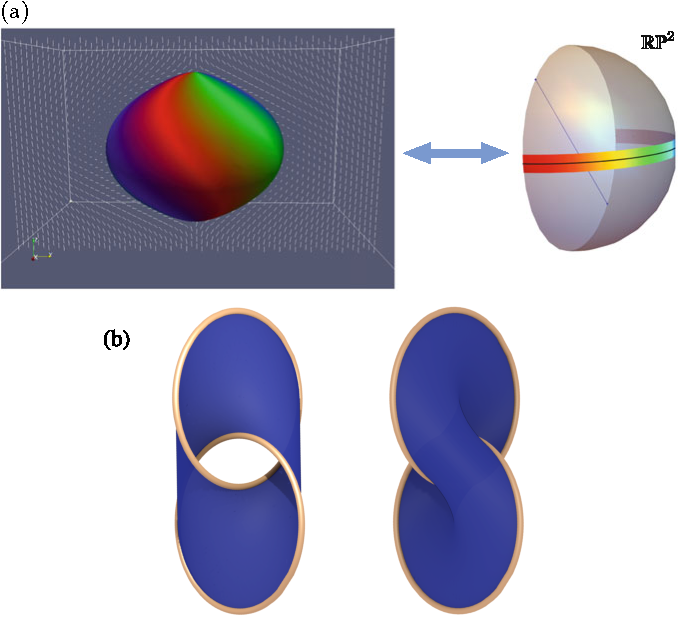
\includegraphics[width=0.8\linewidth]{\IntroductionFigures/PontryaginThom.pdf}
\caption{hi }
\label{fig:PT}
\end{figure}
\subsection{Beyond disclination lines}
The above sections focused on the knotting and nontrivial topology of disclination lines --- defects in the director $\bf n$ itself. Given the experimental focus on systems of this kind, and their direct connection to the idea of a knotted field, this is natural. However even in the absence of defects liquid crystals support an array of topological phenomena which may also be considered examples of knotted fields, although perhaps in a different sense to those discussed above. 

\subsubsection{Skyrmions and Hopfions}
The most well known topological feature of this kind is a skyrmion, an example of which is shown in figure \ref{fig:HopfionMontage}(a) given by the vector field ${\bf n}(r) = \cos(\pi r) {\bf e}_z + \sin(\pi r) {\bf e}_r$ on the unit disk. Fixing the director on the disk boundary, we may wrap this texture around a sphere (compactifying the boundary to a point) at which point its toplogy is captured by a map ${\bf n} : S^2 \rightarrow S^2$, in other words an element of $\pi_2 (S^2)\approx \mathbb{Z}$. These textures are a well studied feature of vector and line fields in two dimensions \citep{AlexanderBook}. We are primarily interested in the properties of order in three dimensions, and as such focus on their three dimensional `cousins': Hopfions.
\begin{figure}[htbp]
\centering
\includegraphics[width=\linewidth]{\IntroductionFigures/HopfionMontage.pdf}
\caption{hi }
\label{fig:HopfionMontage}
\end{figure}
An experimental image of a Hopfion is shown in figure \ref{fig:HopfionMontage}(b)\citep{ChenThesis,Chen2013}. The figure shows a nematic liquid crystal texture inside a three dimensional cell, where the PT surface has been constructed by extracting director orientation via three-photon fluorescence microscopy. What qualifies the Hopfion as a knotted field becomes clear on viewing this surface: each stripe of colour twists about a torus, linking each other colour exactly once --- in a Hopf link, no less. Skyrmions are classified by an element of $\pi_2(S^2)$. Hopfions are instead classified by $\pi_3(S^2)$, the third homotopy group of the sphere. Heinz Hopf famously showed that $\pi_3(S^2) \approx \mathbb{Z}$, and in doing so constructed an explicit example of a nontrivial element of this group --- the celebrated Hopf Fibration. For mathematical detail on the construction of the fibration we refer to the reader to Refs. \citep{AlexanderBook,BottTuBook}, and for an excellent video of its structure we urge the reader to consult Ref.~\citep{Johnson2011}. Figure \ref{fig:HopfionMontage}(b) shows an experimental image of this fibration; the energetics of the liquid system favour a fixed far field nematic direction, mimicking the skyrmion boundary conditions and allowing the domain to be compactified $\mathbb{R}^3\rightarrow {S}^3$. The nematic texture then realises a map $\n: S^3 \rightarrow \mathbb{R}P^2$, and $\pi_3(\mathbb{R}P^2) \approx \pi_3(S^2) \approx \mathbb{Z}$. The fact that the order lies in $\mathbb{R}P^2$ not $S^2$ is reflected in that fact that there are two stripes of each colour on the experimental fibration~\citep{Chen2013,Ackerman2017}; in figures \ref{fig:HopfionMontage}(c,d) we show a hopfion in vector order, containing only single stripes, with two particular stripes picked out to make the linking clear.
\subsubsection{The geometry of vector fields}
The linking of inverse images is the hallmark of the hopf texture (figure \ref{fig:HopfionMontage}(e)). However without data processing, this linking is not an immeadiately apparent feature of the director. By contrast the knotted disclinations, and even their associated PT surface, in figure \ref{fig:KnottedLiquidCrystal} may be clearly visualised. This is a consequence of the coupling of these topological features to the geometry, energetics and ultimately interaction with light of the liquid crystal, a coupling not present in the inverse images charecterising the Hopfion. This observation invites the question: are there `natural' features of the Hopfion, or nonsingular liquid crystal textures in general, which can be used to infer their topology? We will explore this question, with a particular focus on a recent discovered phase of liquid crystal, in \S\S\ref{ch:3}. The focus will be on naturally geometric structures inside the liquid crystal which also contain some topological information, and so we now discuss the geometry of liquid crystals, and vector fields more generally. 

The fundamental geometry and energetics of nematics was encoded by Frank in 1958~\citep{Frank1958}, where he gave a free energy for their elastic distortions. We give this free energy here in a slightly nonstandard form, following Ref.~\citep{Selinger2019}:
\begin{equation}
    F = \int d^3 {\bf r} \quad \frac{K_1}{2} (\nabla \cdot {\bf n})^2 +\frac{K_2}{2} ({\bf n} \cdot \nabla \times {\bf n})^2 +\frac{K_3}{2}({\bf n} \cdot \nabla) {\bf n} + \frac{K_{24}}{2} \mathrm{Tr}(\Delta)^2,  
    \label{eq:Frank}
\end{equation}
\begin{figure}[htbp]
\centering
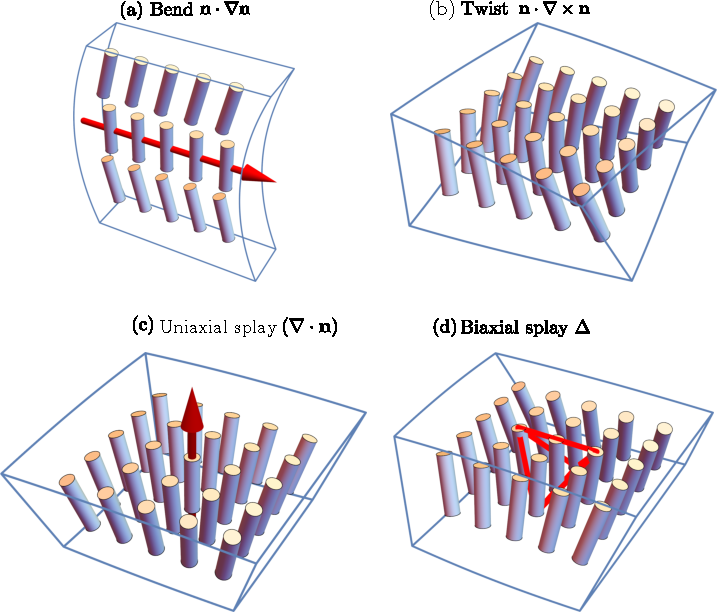
\includegraphics[width=0.7 \linewidth]{\IntroductionFigures/FrankFreeEnergy.pdf}
\caption{hi }
\label{eq:FrankFreeEnergy}
\end{figure}
where the various $K_i$ are elastic constants\footnote{These constants do not match one-to-one with those found in the standard writing of the Frank free energy; see Ref.~\citep{Selinger2019}.}. Each term in eq. \ref{eq:Frank} comes from a different mode of distortion for the liquid crystal, shown in figure (\ref{fig:FrankFreeEnergy}):
\begin{eqnarray}
    &({\bf n} \cdot \nabla) {\bf n} \quad \mathrm{Bend},\\
    &{\bf n} \cdot \nabla \times {\bf n}\quad \mathrm{Twist}, \\
    &\nabla \cdot {\bf n}\quad \mathrm{Uniaxial}\ \mathrm {Splay}, \\
    &\Delta(\bullet) := \frac{1}{2}\Big((\bullet \cdot \nabla {\bf n})+\bf n \times({\bf n \times \bullet \cdot n)\Big)\quad \mathrm{Biaxial}\ \mathrm {Splay}. 
\end{eqnarray}
Vector order has a local rotational symmetry under which the free energy eq. (\ref{eq:FrankFreeEnergy}) must remain invariant, and indeed the above terms are exactly those combinations of gradients which respect this symmetry. More precisely, the terms appearing in eq. (\ref{eq:FrankFreeEnergy}) correspond to the magnitudes of the irreducible representations of $\nabla{\bf n}$ under the action of the rotation group $SO(2)$. These piece together to give a decomposition of $\nabla {\bf n}$ which is naturally written in terms of gradients parallel and perpendicular to the director, $\nabla {\bf n}=\nabla {\bf n}_\parallel + \nabla {\bf n}_\perp$, where
\begin{eqnarray}
    &\nabla {\bf n}_\parallel=  {\bf n}^* \otimes ({\bf n} \cdot \nabla) {\bf n}\\ 
    &\nabla {\bf n}_\perp= \frac{\nabla \cdot {\bf n}}{2}I - \frac{{\bf n} \cdot \nabla \times {\bf n}}{2} J + \Delta .
    \label{eq:GradientDecomposition}
\end{eqnarray}
$I$ is the identity transformation, and $J= \bf n \times \bullet$ is rotation about $\bf n$.\footnote{That the twist and splay terms appear squared in eq. \ref{eq:FrankFreeEnergy} is because the decomposition eq. \ref{eq:GradientDecomposition} is for vector order, not nematic order. The additional symmetry $\bf n \sim -n$ forces us to square these terms.}. The geometry of $\nabla \bf n_\perp$ and $\Delta$ in particular has been explored in Ref. \citep{Machon2016b}. $\nabla \bf n_\perp$ describes how $\bf n$ varies as one moves in a plane perpendicular to it; this is a classical object in differential geometry of surfaces called the shape operator. The decomposition eq.~\ref{eq:GradientDecomposition} corresponds to its breakdown into an isotropic piece $I$, an antisymmetric piece $J$ and a traceless symmetric piece $\Delta$ (if $\bf n$ were the normal to a family of surfaces the antisymmetric piece would vanish). All directional information is contained in $\Delta$; its eigenvectors coincide with those of $\nabla_\perp \bf n$ and pick out the two directions of principal curvature in plane perpendicular the director. This explains the name `biaxial splay' for its mode of distortion. The geometry of $\nabla \bf n_\parallel$ is less well explored. It describes the bending of the director field: if one traces a single curve to which $\bf n$ is tangent, then $\nabla \bf n _\parallel$ gives the classical curvature from the differential geometry of space curves \citep{DoCarmoBook}. A more complete account of its geometry will in part be the topic \S\S\ref{ch:3}.
 
Each of the pieces in \ref{eq:GradientDecomposition} is manifestly geometric, but they also represent topological information, as canonical sections of vector bundles defined by the director. At each point in the material, the director $\bf n$ splits the tangent space into a line parallel to $\bf n$, $L_n$, and a plane perpendicular to it, $\xi$, $T \mathbb{R}^3 \approx L_n \oplus \xi$. An example of this splitting is shown in figure \ref{fig:SplittingMontage}. The families of lines $L_n$ and planes $\xi$ vary smoothly with the director, and such smoothly varying families of vector spaces are called vector bundles \citep{TuBook,MilnorStasheffBook}. The most famous example of a vector bundle, and the interesting properties they can have, is the family of planes tangent to $S^2$ (its tangent bundle). The Poincare-Hopf theorem tells us one cannot `comb a sphere' \citep{Milnor1997}, in other words one cannot choose a nonzero tangent vector everywhere on the sphere. Said more technically, one cannot find an everywhere nonzero section of the tangent bundle to the sphere. This failure is connected to the topology of $S^2$; if one sums the windings of all the zeros in the vector field one obtains the Euler Characteristic of $S^2$. An entirely analogous result holds for any vector bundle; the zeros of a section of a vector bundle encode its Euler Class \citep{BottTuBook, MilnorStasheffBook}. Returning to eq.~\ref{eq:GradientDecomposition}, $\nabla_\perp \bf n$ is a section of the bundle $\xi^* \otimes \xi$ --- it maps vectors orthogonal to $\bf n$ into vectors orthogonal to $\bf n$ --- and the bend $\nabla_\parallel \bf n$ is a section of the bundle $L_n^* \otimes \xi$. Both probe the topology of $\xi$ and, loosely speaking, as $\xi$ is in one-to-one correspondance with the director $\bf n$ this topology carries over to $\bf n$. The zeros of $\Delta$, called umbilic lines in analogy to the umbilic points of the differential geometry of surfaces, have been investigated in Ref.~\citep{Machon2016b}. The zeros of $\nabla_{\parallel} \bf n$, which we will call $\beta$ lines, will be the subject of \S\S\ref{ch:3}.
\begin{figure}[htbp]
\centering
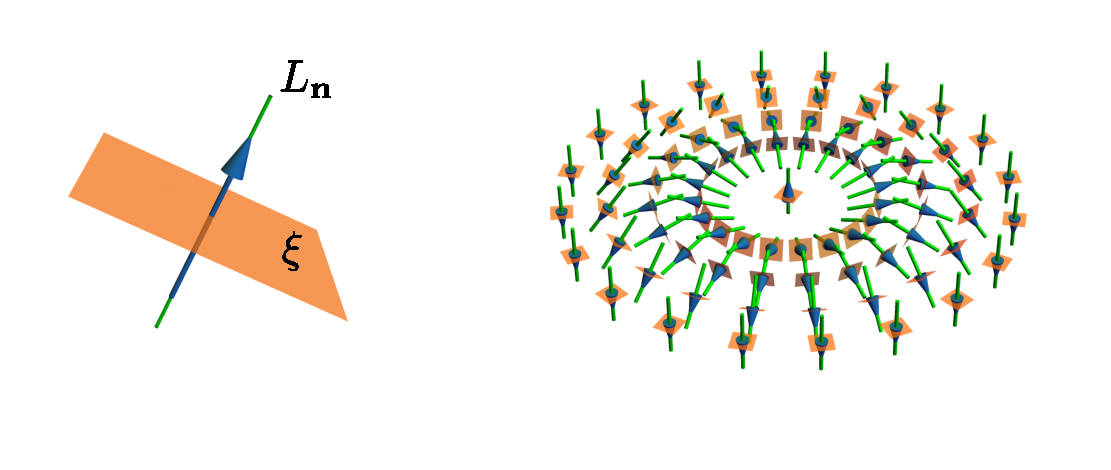
\includegraphics[width=\linewidth]{\IntroductionFigures/SplittingMontage.pdf}
\caption{hi }
\label{fig:SplittingMontage}
\end{figure}

The umbilic and $\beta$ lines are natural geometric structures found in any vector field. However, they assume a particular relevance when strongly coupled to the energetics of the liquid crystal texture. One way to do this is to frustrate the liquid crystal with boundary conditions, as in the disclinations of figure \ref{fig:KnottedLiquidCrystal}. Another is to pass to different phase of liquid crystal, where such coupling exists. In the case of umbilic lines, this setting is the cholesteric phase \citep{Bellar2014}, in which the liquid crystal has a preference for nonzero twist; $\Delta$ turns out to be related to the axis of this twisting \citep{AlexanderBook}, and its zeros thus encode energetic frustration inside the cholesteric \citep{Machon2016b}. For $\beta$ lines, the natural setting is a recently discovered phase of liquid crystal, the twist-bend or splay-bend nematic \citep{Lavrentovich2018}. These materials, comprised of banana shaped molecules, have an energetic preference for everywhere nonzero bend. A second focus of \S\S\ref{ch:3} will be on this interplay between geometry and energetics in twist-bend nematics. 

\section{Modern knotted fields: Excitable Media}

\setlength{\epigraphwidth}{5in} 
\epigraph{``In excitable media we may have a new context in which something like a vortex atom theory can live again, strangely transfigured.''}{A. T. Winfree, The Geometry of Biological Time, Chapter 9.}
\begin{figure}[htbp]
\centering
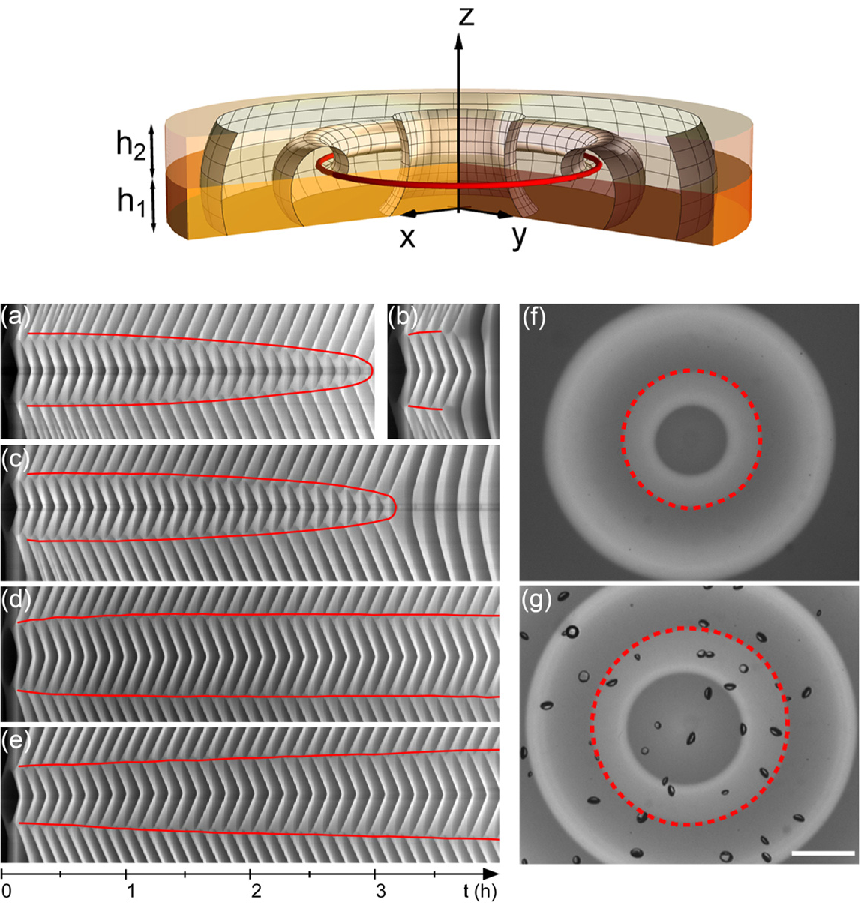
\includegraphics[width=\linewidth]{\IntroductionFigures/FNExperimental.pdf}
\caption{hi }
\label{fig:FNExperimental}
\end{figure}

We now come to our final example of knotted fields, those found in excitable media. We might have discussed them immeadiately after fluids and superfluids, and indeed we will see closer similarities to those systems than to liquid crystals. That we choose not to is a reflection of their relative lack of experimental development. By way of prelude, the modern state of affairs in these systems is that the analogy to a fluid vortex ring can be generated experimentally. Figure \ref{fig:FNExperimental}(a) shows a schematic of a thick dish of the Belousov-Zhabotinksy reagent, a medium which support waves of propogating chemical activity. Axially symmetric waves of such activity spiral outwards from a  `singular' ring shown in red --- exactly what is occuring on this ring will be discussed below. Figure \ref{fig:FNExperimental}(b) shows an experimental realisation of this setup, viewed from the side in figures (a)--(e) and from the top in (f)--(g). From the side the ring appears as a discontinuity in the emitted wavefronts, with a second such discontinuity where the fronts collide in the middle of the dish. The overlaid red curves track the position of this ring. They show, firstly, that it stably persists over several hours, and secondly that it has its own dynamics, expanding, contracting or reaching a stable radius (the outcome may be experimentally tuned). The topological possibilities, dynamics, and organisation of the entire excitable medium by these rings are the subject of this section, and of \S\S \ref{ch:3}. Such rings have not been experimentally tied in nontrivial confugrations, but proposals exist \cite{Sutcliffe}. As we shall see in this section, such an experiment would be extremely interesting.

\subsubsection{Excitable media}

The building block of an excitable medium is an excitable oscillator, something which rests in a quiescent locally stable state but which, given a small kick, becomes excited before relaxing back to quiescence. A prototypical example is a nerve cell. Given an electrical input, the cell `fires', becoming excited, before slowly relaxing back to its resting state where it can be triggered again. An excitable medium is a continuum of these oscillators, all coupled together, in our case by diffusion of activity from one oscillator to its spatial neighbours. Such media support waves of activity, where an excitation in one oscillator triggers its neighbours to `fire' also. A pleasing example of such waves is a grass fire \cite{Winfree1983}. The oscillators are blades of grass. Their resting state is unburnt, their excited state burnt. After burning, the blades slowly grow back, able to be burnt again. A field of grass, the excitable medium, supports a wave of excitation, i.e. a moving  front of grass fire. Note the front has a leading edge (the transition from unexcited to excited) and a trailing edge (the transition from excited to unexcited).

There is an enormous experimental and theoretical literature on systems exhibiting this sort of behaviour; for references see \citep{WinfreeBook}. We present a minimal mathematical model, which shall be the focus of \S\S\ref{ch:2}, and which provides an effective description of many more complex excitable media \citep{WinfreeBook}: the Fitzhugh-Nagumo model \cite{Fitz}
\begin{eqnarray}
&\frac{\partial u}{\partial t}= \frac{1}{\epsilon}(u - \frac{1}{3} u^3 - v) + \nabla^2 u, \\
&\frac{\partial v}{\partial t} = {\epsilon}(u + \beta - \gamma v).
\label{eq:FN}
\end{eqnarray}
Here $u(\bf {x} ,t)$ , $v({\bf x},t)$ are two real valued scalar fields, with $\epsilon,\gamma,\beta$ model parameters. The coupling which turns this system from an excitable oscillator to an excitable medium is through diffusion $\nabla^2 u$, in this instance in the $u$ variable only (although variants with diffusion in each variable also exist). The phase plane for the ODE system without diffusion is shown in figure \ref{fig:FN}(a), with parameter choices which will generate an excitable oscillator. The system has a fixed  point $(u^*,v^*)$ (black dot), but given a finite perturbation in $u$ it will execute a large loop in phase space, jumping to the upper branch of the $u$ nullcline, crawling along it until the first inflection, whereupon it jumps to the lower branch and crawls again back to the fixed point (black arrows in the figure). In the sense that a perturbation in $u$ instigates this loop, $u$ might be considered an `excitor' variable and $v$ a `recovery' variable.
\begin{figure}[htbp]
\centering
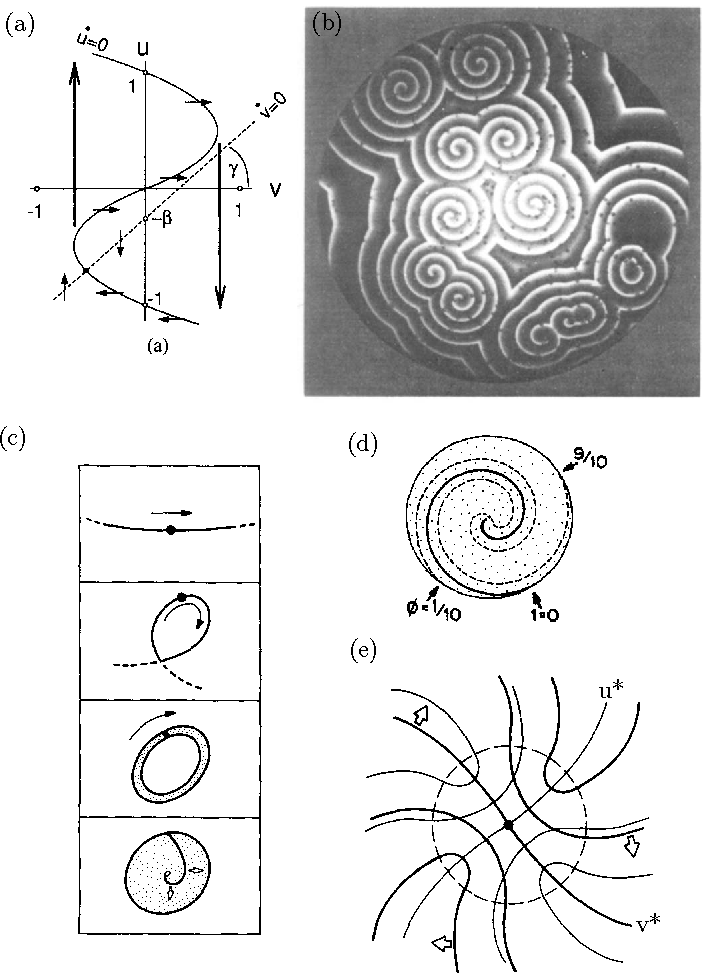
\includegraphics[width=\linewidth]{\IntroductionFigures/FN.pdf}
\caption{hi }
\label{fig:FN}
\end{figure}

\subsubsection{The topological possibilities of excitable media}

The key topological observation is that the excitation-recovery loop is a circle $S^1$. In a portion of excitable media $M$, the state of a typical point lies somewhere on this loop, and thus we can describe the system with a map $\phi : M \rightarrow S^1$, a situation encountered before in superfluids. Concretely mapping between $(u,v)$ and $\phi$ may be achieved via something of the form $(u,v) = (2 \cos \phi - u^*, \sin \phi - v^*)$, stretching $S^1$ over the excitation-recovery loop. That the system is charecterised by the phase field $\phi \in S^1$ immeadiately implies the potential existence of knotted and linked vortices if our domain $M$ is three-dimensional, again by simple analogy with superfluids. What makes this system so interesting is that the character and dynamics of these phase singularities are very different to what we have encountered before. 

In two dimensions these singularities are at the core of spiral waves, a collection of which are shown in the Belosuv-Zhabotinksky reagent in figure \ref{fig:FN}(b). The anatomy of a single spiral wave is dissected in figure \ref{fig:FN}(c)--(e). In figure \ref{fig:FN}(c), one imagines taking an initially thin ring of excitable medium and setting a wave of excitation running around it. If the ring is thickened, we expect some spatial variation in the wavefront--- it turns out that given isotropic diffusion in eq. \ref{eq:FN} it takes the shape of an involute spiral started from the inner edge of the annulus \citep{WinfreeBook}. This thickening process happily continues until the time taken for the inner edge of the wave to circulate once is comparable to the recovery time of the medium, a condition which defines a `core region', inside of which the $(u,v)$ states of points leave the excitation-recovery loop and so cannot be reliably assinged a phase $\phi$ (this is analogous to what happens inside the healing lengthscale which sets vortex core size in superfluids). A phase description in which the core is idealised to zero radius is shown in figure \ref{fig:FN}(d), and a qualitative picture of the corresponding contours of $(u,v)$ is shown in figure \ref{fig:FN}(e). These `rotors' periodically emanate waves of excitation which organise the entire medium, splitting it into domains separated by shock structures where two wavefronts coincide and annhiliate (figure \ref{fig:FN}(b)).

TODO: SOMETHING ABOUT LENGTH AND TIMESCALES

\begin{figure}[htbp]
\centering
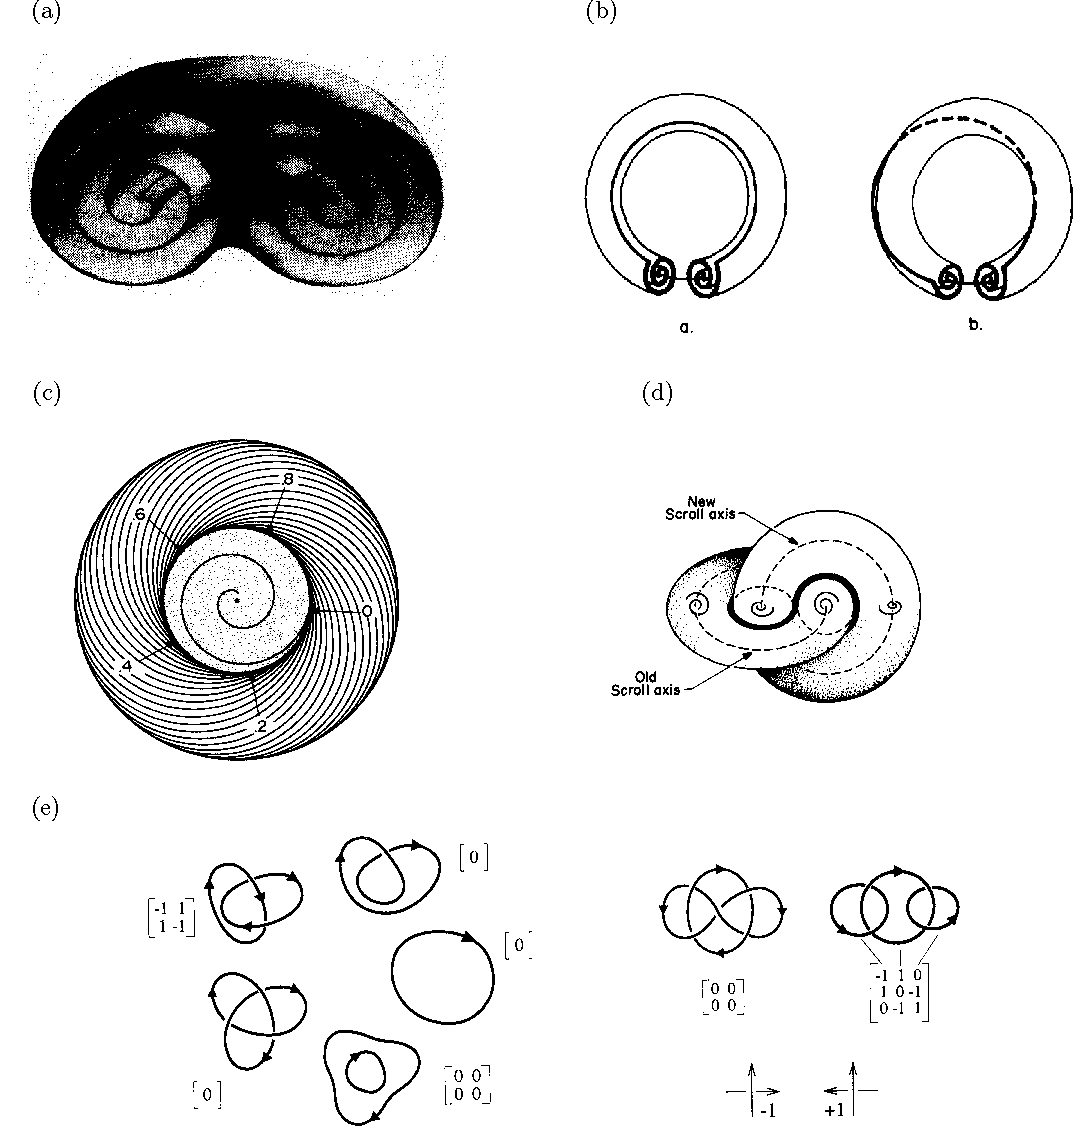
\includegraphics[width=\linewidth]{\IntroductionFigures/FN3D.pdf}
\caption{hi }
\label{fig:FN3D}
\end{figure}

In three dimensions, we have a linelike phase singularity, a vortex filament, emitting `scroll waves'. The geometric and topological possibilities of linked and knotted vortex filaments were first investigated in a series of papers by A.T. Winfree and S. Strogatz \citep{Winfree1983, Winfree1983b, Winfree1983c, Winfree1984}. The simplest possibility is for filament to close into a ring, emitting axially symmetric waves which fill space as shown in figure \ref{fig:FN3D} (a). This is the scenario was encountered experimentally in figure \ref{fig:FNExperimental}. However, Winfree and Strogatz demonstrated numerous other possibilities. For example, we once again have internal structure along the singularity, in this case the phase of rotor in succesive cross sections along the filament, which opens up the possibility of self linking. The simplest such scenario, a twisted scroll wave, is shown in figures (b) and (c). Focusing on figure (c), we note that such twisting implies a full cycle of phase about a line threading the hole in the ring. In other words, a second phase singularity must exist along this line too! Closing this line into a second loop, we obtain figure (d); two scroll rings, each with linking and self linking number (+)1. Winfree and Strogatz extend this line of reasoning in a manner familiar to that of Moffatt \citep{Moffatt1969} to derive a topological selection rule on allowed configurations of knotted vortices: 
\begin{equation}
    0 = \sum_{i,j, i\neq j} Lk(C_i,C_j) + SL(C_i) \quad \forall i. 
    \label{eq:SelectionRule}
\end{equation}
This rule has a similar feel to the helicity count of eq. (\ref{eq:HelicityCount}), but its content is slightly different. It is a condition each knotted loop in a link must satisfy in order for the whole to exist. We note briefly that one might be tempted to use eq.~(\ref{eq:SelectionRule}) as a basis for a definition of Helicity in excitable media. In fact a continuum definition of a helicity has been given \citep{Trueba2009} but it is currently not clear (to me at least) 
how the concepts interlink; it is an interesting question for further study.

\subsubsection{The dynamical possibilities of excitable media}

Provided the topological constraint eq.~(\ref{eq:SelectionRule}) remains satisfied, there is no reason link reconnections cannot occur, as they do in the other systems we have discussed. In figure \ref{fig:FN3D}(e) we show two groups of allowed knotted vortices, and within each group transmutations are topologically allowed. As Winfree and Strogatz note, questions of whether or not they actually occur in a given excitable medium ``probably depend sensitively on the exact kinetics of the medium'' \citep{Winfree1984}. For example, in the experiment of \ref{fig:FNExperimental}(b)  \citep{Totz2015} we saw that these vortex lines are not merely static emitters of wavefronts, they have their own dynamics, and one has no \emph{a priori} reason to expect these dynamics to preserve topology. What is absolutely remarkable is that, in a certain parameter regime in the FitzHugh-Nagumo model, it was found that they do \citep{Winfree1990,Henze1993}. Using $\epsilon = 0.3, \beta = 0.7, \gamma=0.5$, a stable vortex ring was found in \citep{Courtemanche1990}, shown in figure \ref{fig:FNKnots}(a), followed by a stable trefoil knot \citep{Henze1991}(in a slightly different kinetics) and then a variety of apparently stable knots and links \citep{Henze1993} summarised in figure \ref{fig:FNKnots}(b). An account of this first period of development may be found in Refs.~\citep{Winfree1990, WinfreeBook,WinfreeChapter}. Subsequent work \citep{Sutcliffe2003} confirmed a wide basin of stability for the trefoil knot and the Hopf link over substantially larger time periods than the original trefoil simulations were run for. More recently, Maucher and Sutcliffe \citep{Maucher2016} showed that the FitzHugh-Nagumo dynamics is even capable of simplifying a tangled unknot into a unique canonical round form and demonstrated stable forms for more complex knots --- the figure-eight and torus links in certain geometries \citep{Maucher2017}. A simplification of a 13 crossing knot is shown in figures \ref{fig:FNKnots}(c), with a cross section to show the associated wavefield in figure \ref{fig:FNKnots} (d) (one might compare to figure \ref{fig:FN}(b)). The stable torus and figure-eight knots with associated minimal lengths are shown in figure \ref{fig:FNKnots}(e).
\begin{figure}[htbp]
\centering
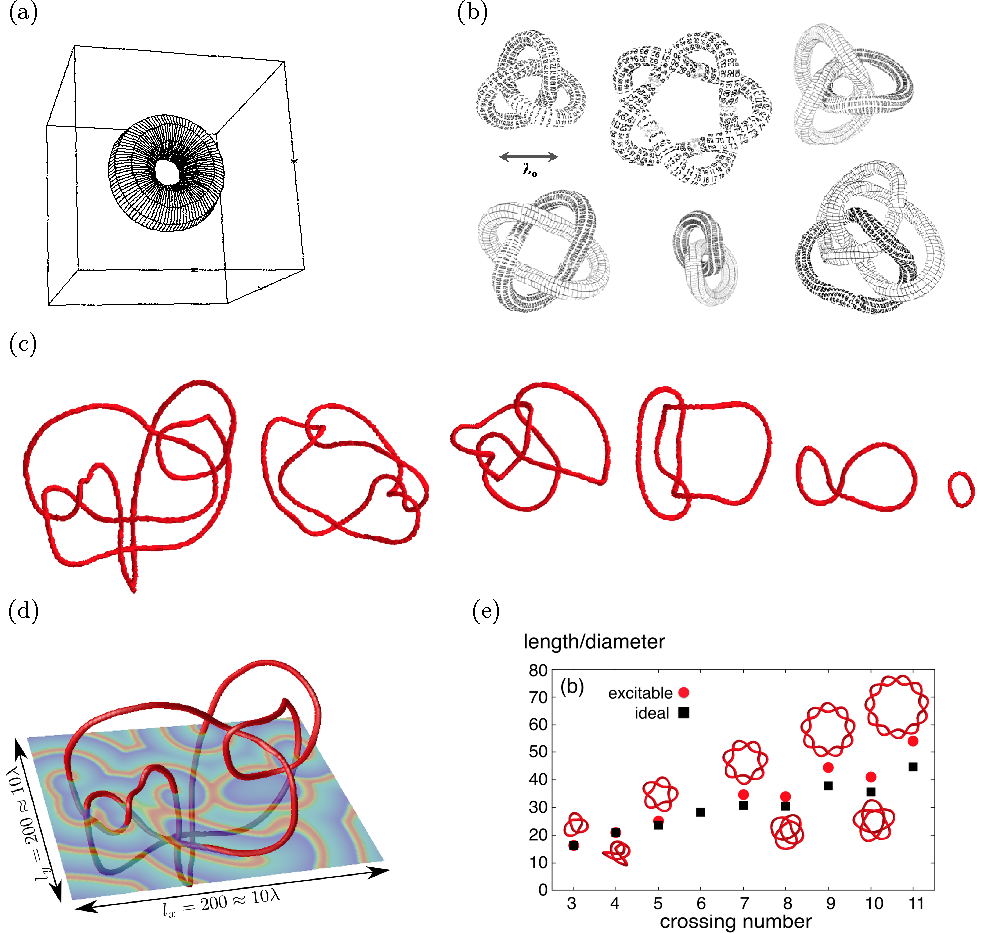
\includegraphics[width=\linewidth]{\IntroductionFigures/FNKnots.pdf}
\caption{hi }
\label{fig:FNKnots}
\end{figure}
These numerical findings are in stark constrast to what we saw in fluids, superfluids and liquid crystals (indeed, in most knotted fields), and invite a series of questions: What determines the dynamics of these vortices? How are reconnections avoided? What is the mechanism of knot untangling? Are all knots stable, and if so can we predict their shapes? In some form these questions have existed since the first knotted vortices were discovered. Initial theoretical work focused heavily on the idea that their laws of motion could be explained by a `local geometry hypothesis' \cite{Win} in which dynamics at each point on the curve were governed by some local law of motion involving its cuvature, the twist of spiral wave phase etc. After a perturbative theory for such a law was developed~\cite{win}, substantial work went into testing whether or not this was the case~\cite{win}, of which an account may again be found in \cite{win}. Summarising very coarsely, such laws found some success in describing isolated filaments, but of course encounter problems whenever interfilament interactions are required. The problem is that evidence ultimately suggested such interactions were integral to describing stable knots \cite{Henze}, and as such a local geometry hypothesis failed to account for their dynamics. The observed untangling without reconnection of unknots shown in figure \ref{fig:FNKnots}(e) \cite{} further casts doubt on whether such a law could be made to work. 

We remark that the idea of reducing the dynamics of an entire field to that of a curve is not unique to excitable media, but cuts across knotted fields. In particular the idea is similar to the Local Induction Approximation (LIA) in fluids and superfluids \cite{Saffman}, in which the Biot-Savart law of motion governing vortex lines is approximated by a dominant contribution arising from local curvature, which leads to motion binormal to the curve --- in the case of a vortex ring, drift perpendicular to the plane it lies in, a feature shared by the rings studied here \cite{}. Further, exact knotted solutions to the LIA \emph{do} exist \cite{Kida,Hasimoto}, and one might have hoped something similar applied here. Note however that the LIA breaks down in fluids too \cite{}, and further that the nature of the fields surrounding the vortices is quite different between the two cases. One crucial difference, as we shall see, is that in excitable media waves propogate without attenuation for potentially arbitrary distances, making a theoretical decoupling of distant segments of the knot difficult.     

In summary, the questions posed above are not satisfactorily answered. Our attempts to explore them, with a focus on systematically testing knots for stability and exploring the importance of nonlocal filament interactions, form \S\S \ref{ch:2}. The potential for experimentally accessible, and spontaneously stable, knotted fields is a major motivator for this work.


\section{Structure of this Thesis}

%This thesis is primarily about Soft Matter systems, and these experiments also provide an answer to the question ``why Soft Matter?''. Soft Matter systems may be loosely chareceterised as those for which geometry plays a fundamental role in their description, and which may undergo substantial deformations in reponse to external forces, changes in temperature etc. The two systems described above, fluids and liquid crystals, are prime examples. Such systems have several appealing features. As we have seen, they are often experimentally accessible, and within the world of soft matter we find a rich diversity of types of order. For example, Refs.~\cite{Tkalec2011,Tasinkevych2014,Copar2015} use the simplest mesophase of liquid crystal, the nematic, however many other types of order are possible \cite{DeGennes}: in \ref{ch3} we study a recently discovered phase, the Twist-Bend nematic \cite{Lavrentovich}, comprised of banana-shaped molcules (in contrast to the rodlike mocules of Figure \ref{fig:LiquidCrystals}). They are described by the director $\bf n$ as in the nematic, but additionally a vector field $\bf p$ describing the local bending of the molecules. As one might expect, this second field $\bf p$ leads to topological features not present in the nematic phase. A more practical motivator, the accessibility of these systems make them candidates for industrial application \cite{Musevic}: witness the ubiquity of Liquid Crystal Display (LCD) screens.
